\chapter{Voltage peak transducer}
\section{Theory and related work} \label{sec:literature_voltage}
A transducer is defined as a device that transforms one form of energy into another form\cite{Neamen:Microelectronics}. AC voltage transducers convert an AC voltage signal to a DC voltage output which is directly proportional to the input signal value. For the purpose of this project, only the maximum value of the input signal is required,hence, the voltage transducer can be implemented using a peak detector circuit.

A standard peak detector usually consists of a diode and a capacitor\cite{Neamen:Microelectronics}. The typical configuration is given in Figure \ref{subfig:simple_peak_detector}. This circuit, however, has the side effect of introducing a voltage drop over the diode. Having an ideal diode that avoids this is thus key to implementing a voltage transducer. This "ideal diode" configuration can be achieved by using a precision rectifier as shown in Figure \ref{subfig:superdiode}. The circuit will perform rectification, similar to a diode, but without introducing a voltage drop\cite{superdiode}. 

The DC voltage output of the transducer is to be sampled by an ADC in an Arduino Beetle board. Thus, it should be amplified to provide sufficient resolution. There are various op-amp configurations for this purpose. The main one that is considered is a difference amplifier, shown in Figure \ref{subfig:difference_amplifier}. As the name suggests, it amplifies the difference between two inputs, one of which is usually a reference/constant signal\cite{difference_amp}.

\begin{figure}
 \centering
     \begin{subfigure}[]{0.45\textwidth}
        \centering
         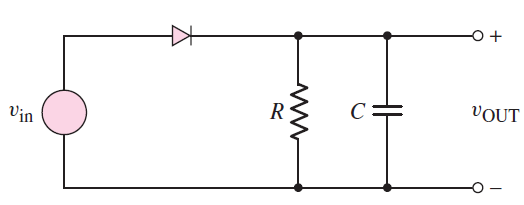
\includegraphics[width=1\linewidth]{./Figures/peak_detector}
		    \caption{Simple peak detector\cite{Neamen:Microelectronics}} \label{subfig:simple_peak_detector}
     \end{subfigure}
      \begin{subfigure}[]{0.35\textwidth}
              \centering
  		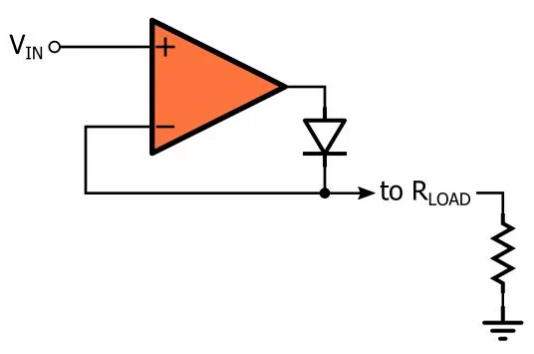
\includegraphics[width=1\linewidth]{./Figures/superdiode}
		    \caption{Precision rectifier circuit\cite{superdiode}} \label{subfig:superdiode}
     \end{subfigure}
     \begin{subfigure}[]{0.35\textwidth} 
             \centering
         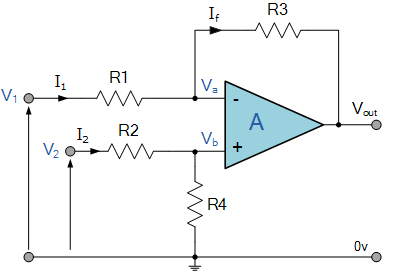
\includegraphics[width=1.\linewidth]{./Figures/difference_amplifier}
		\caption{Difference amplifier\cite{difference_amp}} \label{subfig:difference_amplifier}
     \end{subfigure} 
   \caption{Reference circuits for a voltage transducer.}
    \label{fig:voltage_transducer_theory}
 \end{figure}

\section{Design} \label{sec:design_voltage}

For the purpose of this project, two types of op-amps were provided: a standard TL081 op-amp, and a TLC2272 precision rail-to-rail op-amp. Thus, the first part of the design involves choosing which op-amp to use for each application. Table \ref{tab:op_amp_compare} gives some of the characteristics of both op-amps to aid in this choice.

\begin{table}[h]
        \centering
        \footnotesize
        \caption{TL081\cite{TL081} vs TLC2272\cite{TLC2272}}
         \begin{tabular}{c@{\qquad}rrrr}
          \toprule
             & TL081 & TLC2272\\
          \midrule
          Input voltage             & $\pm\SI{15}{\volt}$        & \numrange{-5.3}{5.0}\si{\volt}  \\
          Common-mode input voltage  & $\pm\SI{1.0}{\volt}$ & \numrange{-5.0}{3.5}\si{\volt} \\
          Differential input voltage & $\pm\SI{30}{\volt}$         & $\pm\SI{16}{\volt}$  \\
          Maximum output voltage           & \SI{4.0}{\volt}              & 4.85V \\
          \bottomrule
        \end{tabular}
     \label{tab:op_amp_compare}
\end{table}

As seen above the rail-to-rail op-amp has a higher maximum common-mode input, as well as output voltage. It also contains 2 op-amps within a single package as opposed to the TL081. For these reasons, it is chosen  for all applications in the voltage transducer, as well as the current and phase shift transducers in Section \ref{sec:design_current} and \ref{sec:design_phase}.

Due to the common-mode specification, the voltage from the transformer must be scaled down before it is input to the precision rectifier. A voltage divider circuit is used to scale down the maximum expected 20VAC signal to a level less than the $\SI{3.5}{\volt}$ common-mode limit.

\begin{equation}
\begin{split}
    V_{in} &\leq \frac{R_2}{R_1 + R_2}V_{max} \\
    0.11 &\leq \frac{R_2}{R_1 + R_2} \\
    R_1 &= \SI{22}{\kilo\ohm}   \qquad R_2 = \SI{1}{\kilo\ohm} \\
\end{split}
\label{eqn:voltage_divider}
\end{equation}

The implemented voltage divider circuit will give an output of 1.23V at 20VAC, which is also within the maximum input voltage limit. The differential voltage can also be calculated as: $V_{d(max)} = (-1.23) - 1.23 = -2.46\si{\volt})$, which is also within the op-amp limits. 

A capacitor can now be chosen for the peak detector circuit. Since the transducer should be accurate to $\SI{150}{\milli\volt}$, the maximum ripple voltage should be less than the expected change in the output for an input change of $\SI{150}{\milli\volt}$. This is given by\cite{Neamen:Microelectronics}: $V_r = \frac{\si{150\milli}}{23} \times 5.6 = \SI{36.52}{\milli\volt}$. As the output stage has a gain of 5.6, the peak detector ripple should be less than $\SI{6.522}{\milli\volt}$. The capacitor can thus be chosen as: $C=\frac{V_{pk}}{fRV_r}=\SI{3.77}{\mu\farad}$. However, for accuracy during sampling, the ripple should be much less than this maximum, so the capacitor is chosen to be ten times larger. Thus, a $\SI{33}{\mu\farad}$ capacitor is chosen.

The second part of the transducer is an output amplification stage. 20VAC should be mapped to 4.5V for maximum resolution, while still leaving room for higher than expected inputs from the transformer. However, on the lower end, 12VAC would not be mapped close to zero if a non-inverting amplifier was used. To try achieve this, a difference amplifier is used. By mapping 10VAC to 0V, the resolution of the circuit is significantly reduced. Looking at the peak detector circuit, 10VAC would map to 0.615V, so, this is set as the reference to connect to the inverting input of the amplifier. To obtain this reference voltage, a voltage divider is connected to the +5V supply. Using a 1k and 10k resistor as shown, the inverting input has a voltage of 0.45V, which is close enough to the designed 10VAC. To calculate the gain of the amplifier, we consider that 1.23V must be mapped to 4.5V. With the current configuration the gain is calculated as 4.5/(1.23-0.45) = 5.77. Using resistors 5.6k and 1k, a gain of 5.6 is achieved.

As a 10-bit ADC is to be used, the resolution is given as 4.883mV/bit. Reversing this to the input of the transducer gives a resolution of 20.05mV/bit. This is much less than our specified accuracy, and allows significant external noise to not affect the circuit operation.

The final voltage peak transducer is given below.
  
  \begin{figure}
        \centering
         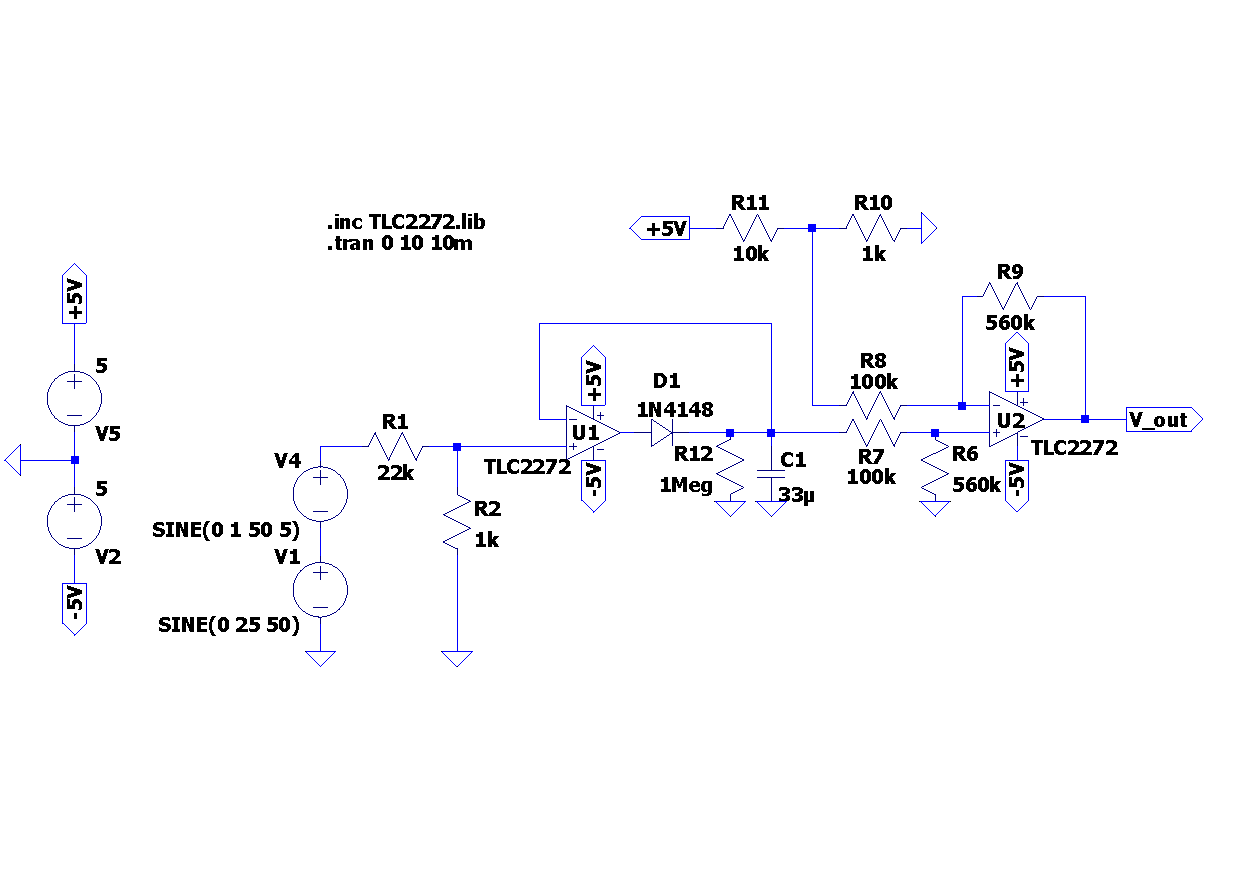
\includegraphics[width=1\linewidth]{./Figures/voltage_circuit.pdf}
		    \caption{Voltage transducer circuit.} \label{fig:voltage_circuit}
 \end{figure}

\section{Simulation} \label{sec:simulation_voltage}

\begin{figure}
        \centering
         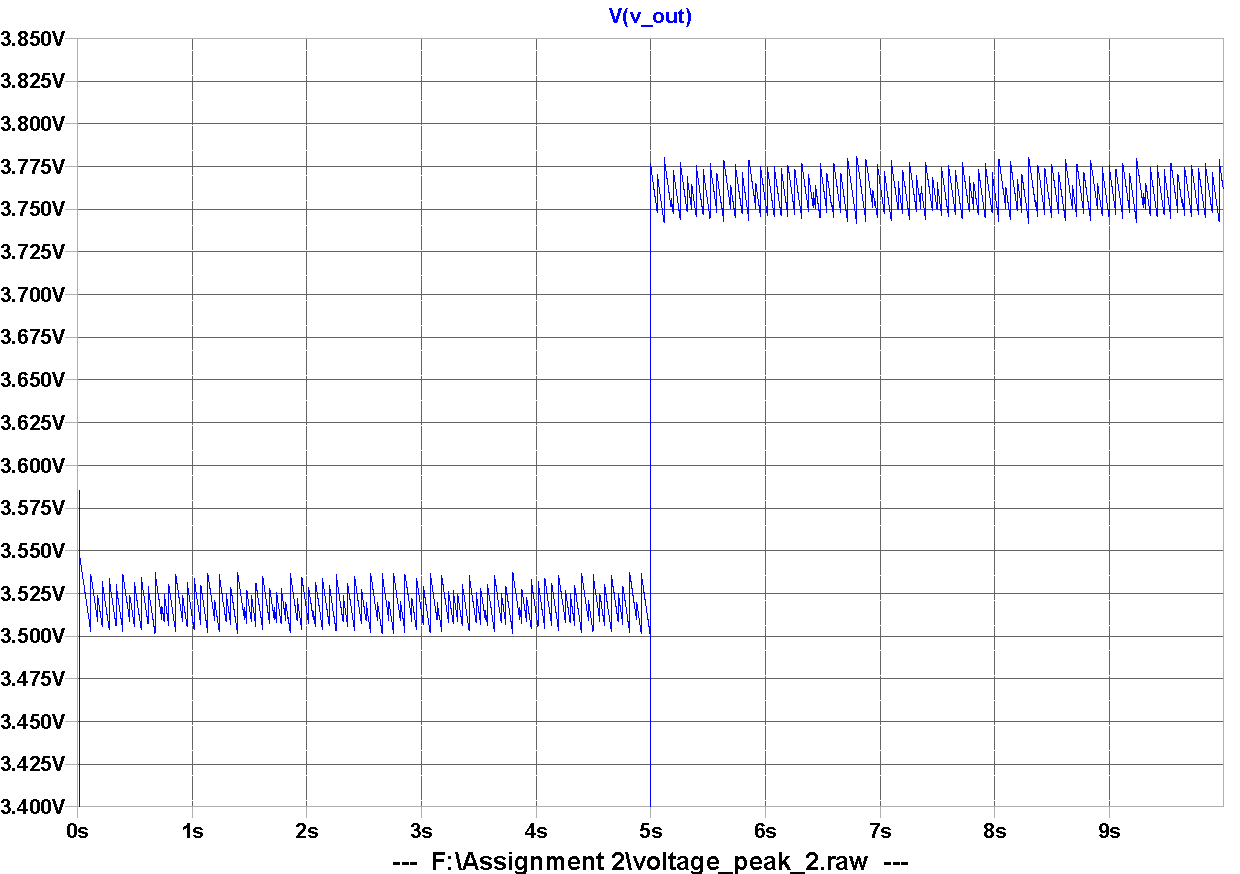
\includegraphics[width=0.75\linewidth]{./Figures/voltage_transducer_simulation}
		    \caption{Voltage transducer circuit.} \label{fig:voltage_simulate}
 \end{figure}
 

\section{Measurements} \label{sec:measurements_voltage}
The deduced input in Tables \ref{tab:voltage_unit_test} and \ref{tab:voltage_integrated_test} is derived from the circuit in Figure \ref{fig:voltage_circuit}.

$V_{out} = (V_{in} \times \frac{1k}{1k + 22k} - 5 \times \frac{1k}{1k+10k}) \times 5.6$
\begin{figure}
 \centering
     \begin{subfigure}[]{0.45\textwidth}
        \centering
         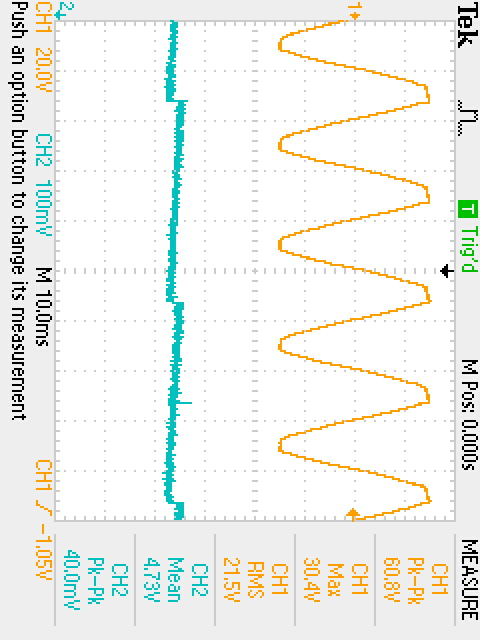
\includegraphics[height=1\linewidth,angle=90]{./Figures/voltage_measure}
		    \caption{AC input and DC output for mid range load.} \label{subfig:voltage_measure}
     \end{subfigure}
      \begin{subfigure}[]{0.45\textwidth}
              \centering
  		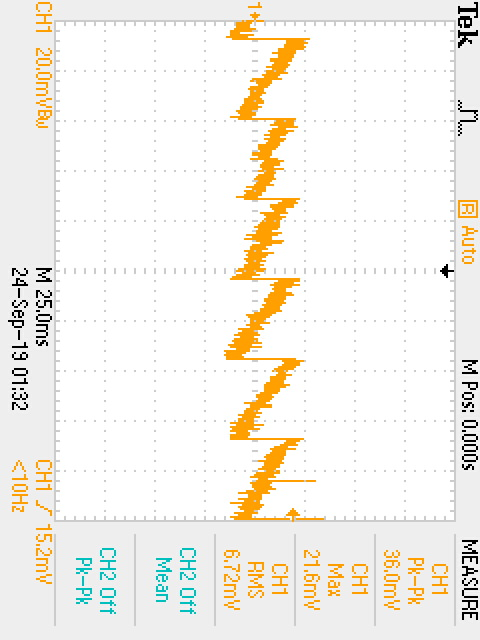
\includegraphics[height=1\linewidth,angle=90]{./Figures/voltage_noise_measure}
		    \caption{Voltage transducer noise levels for a mid sized load.} \label{subfig:voltage_noise}
     \end{subfigure}
 \end{figure}
 
\begin{table}[h]
        \centering
        \footnotesize
        \caption{Voltage transducer unit test results}
         \begin{tabular}{cccccc}
          \toprule
             \textit{\footnotesize Emulated level} & \textit{\footnotesize Signal generator} & \textit{\footnotesize Signal generator} & \textit{{\footnotesize Analogue output}} & \textit{\footnotesize Deduced input} & \textit{\footnotesize Difference}\\
             $[V_{peak}]$ & $[mV_{peak}]$ & $[mV_{peak}]$ & $[VDC]$ & $[V_{peak}]$ & $[mV]$ \\
          \midrule
          16.00 & 695.65 & 712 & 1.40 & 16.41 & 409.9 \\
          21.00 & 913.04 & 932 & 2.65 & 21.3795 & 379.54 \\
          21.15 & 919.56 & 936 & 2.68 & 21.544 & 393.83 \\
          21.30 & 926.09 & 944 & 2.72 & 21.626 & 367.04 \\
          26.00 & 1130.04 & 1180 & 4.03 & 27.006 & 1.006 \\
          \bottomrule
        \end{tabular}
     \label{tab:voltage_unit_test}
\end{table}

\begin{table}[h]
        \centering
        \footnotesize
        \caption{Voltage transducer unit test results}
         \begin{tabular}{ccccccc}
          \toprule
             \textit{\footnotesize Measurement} & \textit{\footnotesize Load R} & \textit{\footnotesize Load C} & \textit{{\footnotesize Measured input}} & \textit{{\footnotesize Analogue output}} & \textit{\footnotesize Deduced input} & \textit{\footnotesize Difference}\\
             & $[\si{\ohm}]$ & $[\si{\mu\farad}]$ & $[V_{peak}]$ & $[\si{\volt}DC]$ & $[V_{peak}]$ & $[mV]$ \\
          \midrule
          No load & open & none & 29.8 & 4.76 & 30.005 & 204.54 \\
          Full load & 100 & none & 28.4 & 4.45 & 28.73 & 331.33 \\
          Mid range & 1k & none & 29.6 & 4.73 & 29.88 & 281.33 \\
          \bottomrule
        \end{tabular}
     \label{tab:voltage_integrated_test}
\end{table}
